%--------------------------------------------CAPA DE ESTRATEGIAS ------------------------------------------------------%

\subsection{Capa de estrategias}
Los elementos de estrategia se utilizan normalmente para modelar la dirección estratégica y las opciones de una empresa, en lo que respecta al impacto en su arquitectura. Se pueden utilizar para expresar cómo la empresa quiere \textbf{crear valor para sus partes interesadas}, las capacidades que necesita, los recursos necesarios para respaldar estas capacidades, así como cómo planea configurar y utilizar estas capacidades y recursos para lograr sus objetivos. Los elementos de estrategia se utilizan para modelar la dirección estratégica y las opciones de la empresa, mientras que los elementos de la capa empresarial se utilizan para modelar la organización operativa de una empresa.

La tabla \ref{tab:Tabla de la capa de estrategia} ofrece una visión general de los elementos de la estrategia, con sus definiciones.\cite{archimate} 

\begin{longtable}{|p{0.15\linewidth}|p{0.45\linewidth}|p{0.2\linewidth} p{0.2\linewidth}|}
    \caption{Tabla de la capa de estrategia}
    \\
    \hline
    \rowcolor[HTML]{AFC5F6} 
    \textbf{Elemento} & \textbf{Descripción} & \multicolumn{2}{c|}{\textbf{Notación}} \\
    \hline
    \endhead
    \hline
    \multicolumn{4}{r}{\textit{Continúa en la siguiente página}} \\
    \endfoot
    \hline
    \endlastfoot
    \label{tab:Tabla de la capa de estrategia}
    %Contenido 1 &
    %\lipsum[1] &
    %Datos A1
    %& Datos B1
    %\\
    %\hline



    Recurso 
    &
    Representa un activo perteneciente o controlado por un individuo u organización. 
    &
\begin{center}
    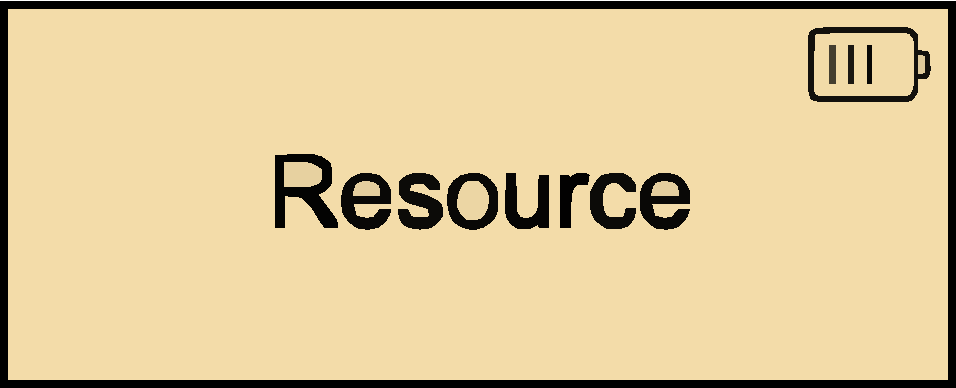
\includegraphics[width=1\linewidth]{imgs/capa_estrategia/fig-Resource-Notation_1.pdf}
\end{center} 
&
\begin{center}
    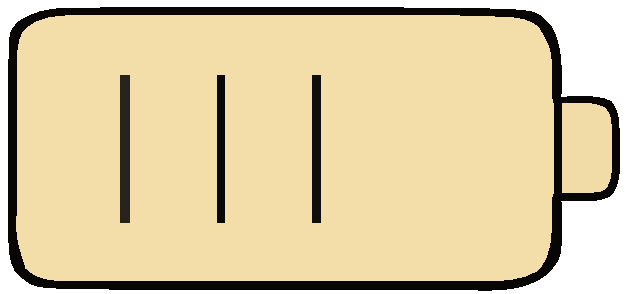
\includegraphics[width=0.8\linewidth]{imgs/capa_estrategia/fig-Resource-Notation_2.pdf}
\end{center}
    \\ \hline



    Capacidad 
    &
    Representa una condición externa o interna que motiva a una organización a definir sus objetivos e implementar los cambios necesarios para alcanzarlos. Representa una habilidad que un elemento activo de una estructura, como una organización, persona o sistema, posee. 
    &
\begin{center}
    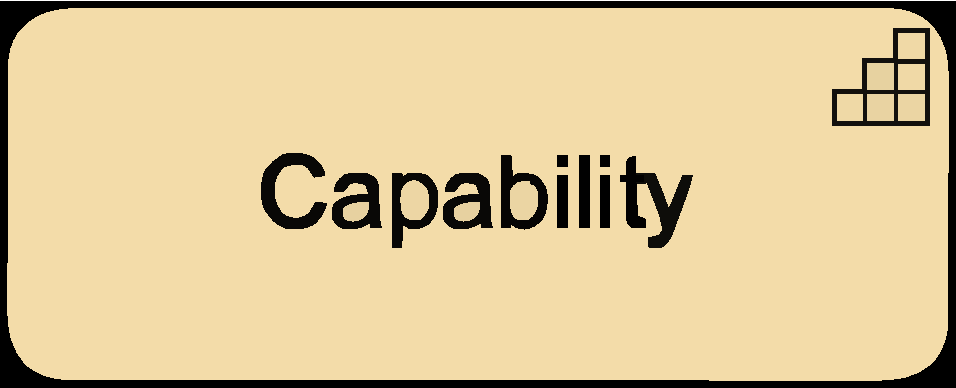
\includegraphics[width=1\linewidth]{imgs/capa_estrategia/fig-Capability-Notation_1.pdf}
\end{center} &
\begin{center}
    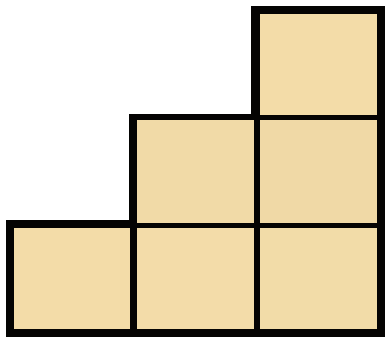
\includegraphics[width=0.5\linewidth]{imgs/capa_estrategia/fig-Capability-Notation_2.pdf}
\end{center}
    \\ \hline



    Transmisión de valor  
    &
    Representa una secuencia de actividades que generan un resultado general para un cliente, stakeholder o usuario final. 
    &
\begin{center}
    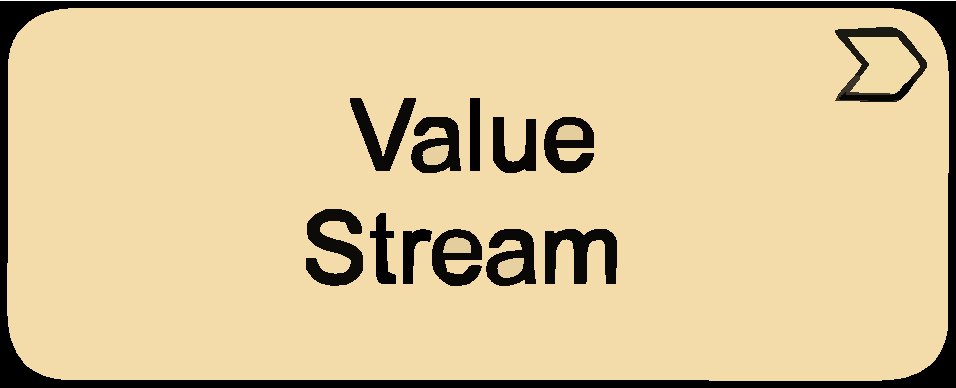
\includegraphics[width=1\linewidth]{imgs/capa_estrategia/fig-Value-Stream-Notation_1.pdf}
\end{center} &
\begin{center}
    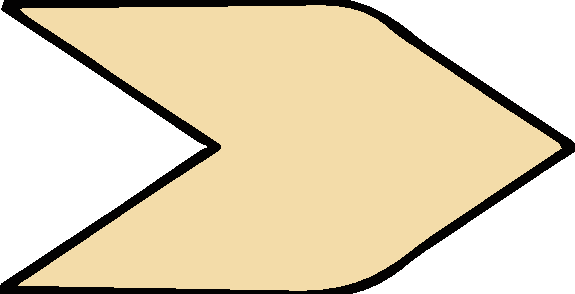
\includegraphics[width=0.5\linewidth]{imgs/capa_estrategia/fig-Value-Stream-Notation_2.pdf}
\end{center}
    \\ \hline



    Curso de acción 
    &
    Representa un acercamiento o plan para configurar algunas capacidades y recursos de la empresa, emprendidos para alcanzar una meta.
    &
\begin{center}
    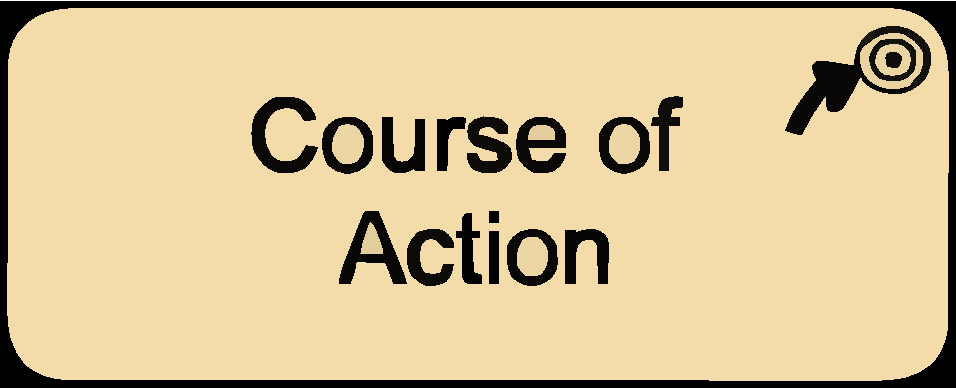
\includegraphics[width=1\linewidth]{imgs/capa_estrategia/fig-Course-of-Action-Notation_1.pdf}
\end{center} &
\begin{center}
    
\includegraphics[width=0.5\linewidth]{imgs/capa_estrategia/fig-Course-of-Action-Notation_2.pdf}
\end{center}
    \\ \hline


\end{longtable}